% !Mode:: "TeX:UTF-8"

\chapter{基于动态温度管理的模型预测控制}

在这一章我们将介绍基于动态温度管理方法的模型预测控制方法。
结合mpc的热模型在\ref{sec:therm_model}节中介绍。2.2节介绍怎么用mpc计算期望的用于引导动态温度管理方法功耗。最后2.3节说明怎么样用mpc计算得到的功耗来引导任务迁移和DVFS。
\section{微处理器热模型}\label{sec:therm_model}
热系统和电路系统是相似的,我们可以用热阻,热容,和等效的热电流电压源来建立微处理器的热模型。
类似于电路系统,$l$ 核的微处理器热模型可以被表达为常微分方程,
\begin{equation}\label{eq:therm_model_cont} 
\begin{split}
G T(t) + C \dot{T}(t) &= B_c P(t),\\
Y(t) &= L T(t),
\end{split}
\end{equation}
其中,$T(t) \in \mathbb{R}^n$ 是表示处理器 $n$ 块温度的向量,包括 $l$个核($l < n$), 边界节点和封装部分的节点;
$G \in \mathbb{R}^{n\times n}$ 包含热阻信息; 
$C \in \mathbb{R}^{n \times n}$ 包含热容信息;
$B_c \in \mathbb{R}^{n \times l}$ 包括功率输入的拓扑信息;
$P(t) \in \mathbb{R}^{l}$ 是 $l$ 个核在时刻 $t$ 的功耗向量,这就是模型的输入;
$Y(t)$ 是 $l$ 个核的温度信息向量,这就是模型的输出;
$L \in \mathbb{R}^{l \times n}$ 是输出选择矩阵,从 $T(t)$ 中选择 $l$ 个核的温度。

为了分析热系统,用欧拉方法或者其他数值积分方法将连续常微分方程 \eqref{eq:therm_model_cont} 离散化为下面的差分方程
\begin{equation}\label{eq:therm_model_disc}
\begin{split}
T(k+1) &= A T(k)+B_d P(k),\\
Y(k) &= L T(k),
\end{split}
\end{equation}
其中,变量 $T(k)$ 、 $P(k)$ 和 $Y(k)$ 是公式 \eqref{eq:therm_model_cont}中
$T(t)$ 、 $P(t)$ 和 $Y(t)$ 的离散形式,  $A$ 和
$B_d$ 是由 $G$、 $C$、 和 $B_c$ 根据离散\eqref{eq:therm_model_cont}的特定的数值积分方法得到的。

对于一般用途, \eqref{eq:therm_model_disc} 中的热模型是用于用芯片上的各单元功耗(即输入$P(k)$)来计算芯片上核的温度(即输出的 $Y(k)$)。

\section{用模型预测控制方法计算期望的功耗}\label{sec:mpc}

\ref{sec:therm_model}节中已经说明,用热模型 \eqref{eq:therm_model_disc}, 可以由给定的功耗输入 $P(k)$ 来计算
芯片上的核的温度 $Y(k)$, 这足以进行热估计和仿真。
对于动态温度管理问题,由给定的功耗来计算期望的功耗也是很重要的,因为动态温度管理方法需要操作功耗方面来管理温度。
有的时候为了简化,可以利用静态热模型由给定的温度信息来计算功耗,静态热模型可以由模型 \eqref{eq:therm_model_cont} 去掉热容项来得到。
然而,基于静态热模型的动态温度管理方法会忽略掉当前热状态,但是当前的热状态在做管理决策的时候非常重要。
这个方法也假设温度和功耗大致温度,这样会影响动态温度管理效用。
为了减轻这个问题,一些反馈控制方案或者优化设计用\eqref{eq:therm_model_cont}中的瞬态热模型(或者\eqref{eq:therm_model_disc}中的离散形式)
在动态温度管理决策时进行更好的功耗计算。
尽管这个方法考虑了当前温度状态而且处理了热与功率的影响,但是这种方法不能得到一个平滑的温度控制。
主要是因为这种方法缺乏未来预测能力,而且只能为温度控制获得当前步的优化功耗。
在这篇文章中,我们用了基于模型预测控制功率计算方法,这个方法将\eqref{eq:therm_model_disc} 中的瞬态热模型扩展成预测形式,它具备为平滑精确热管理计算未来期望功耗的能力。
模型预测控制方法利用\eqref{eq:therm_model_disc} 中的系统模型可以计算得到输入的调整需求,这样就能满足设计者定义的输出。
为了最大化处理器性能,处理器每个核允许的最高温度称作顶温度$Y_{max}$, $Y_{max}$ 通常当做设计者定义的输出来被趋近。
顶温度可以根据现实中的不同应用来被调整,它可以稍微低于处理器允许的最高温度以保证绝对的安全。

首先,我们定义状态和温度变量的差
\begin{equation}
\begin{split}
\Delta T(k) &= T(k) - T(k-1), \\
\Delta P(k) &= P(k) - P(k-1).
\end{split}
\end{equation}
取\eqref{eq:therm_model_disc} 的相邻两步的差,这里有
\begin{equation}\label{eq:diff_model}
\begin{split}
\Delta T(k+1) &= A \Delta T(k) + B_d \Delta P(k),\\
Y(k+1)-Y(k) &= L A \Delta T(k) + L B_d \Delta P(k).
\end{split}
\end{equation}
引入一个新的变量
\begin{equation*}
\hat{T}(k) =
\left[
\begin{array}{c}
\Delta T(k)\\
Y(k)
\end{array}
\right],\\
\end{equation*}
将 \eqref{eq:diff_model} 重写成下面改进的模型
\begin{equation}\label{eq:aug_model}
\begin{split}
\hat{T}(k+1) &= \hat{A}\hat{T}(k) + \hat{B}\Delta P(k),\\
Y(k) &= \hat{L}\hat{T}(k),
\end{split}
\end{equation}
其中
\begin{align*}
\hat{A} &= 
\left[
\begin{array}{cc}
A & 0_m\\
L A & I
\end{array}
\right], &
\hat{B} &= 
\left[
\begin{array}{c}
B_d\\
L B_d
\end{array}
\right],\\
\hat{L} &= 
\left[
\begin{array}{cc}
0_m & I
\end{array}
\right], &
\hat{T}(k) &= 
\left[
\begin{array}{c}
\Delta T(k)\\
Y(k)
\end{array}
\right],
\end{align*}
$0_m$ 是一个合适维度的全零矩阵。


到这里我们已经从\eqref{eq:aug_model}中得到了输入功耗差和输出核的温度之间的关系。
下面,需要确定输入功耗的差来满足核期望的顶温度。假设核未来几个时间步长的顶温度已经给出,写成下面向量的形式
\begin{equation*}
Y_{ceil} = [Y_{max}^T, Y_{max}^T, ..., Y_{max}^T]^T \in \mathbb{R}^{lN_p \times 1}.
\end{equation*}
在这个向量中,$Y_{max} \in \mathbb{R}^{l \times 1}$ 包含每一个核的顶温度。
这里我们假设顶温度不变,这个也符合实际情况,并不是新方法的限制。
$N_p$ 表示从当前到未来$N_p$ 步的时间帧,称作预测域。
为了使核的温度在时间域内趋近于顶温度,将来的控制轨迹(并不知道,需要计算)表示为(当前时刻为 $k$ )
\begin{equation*}
\Delta P_k = [\Delta P(k), \Delta P(k+1), \ldots, \Delta P(k+N_c-1)]^T,
\end{equation*}
其中,$N_c$ 称作控制域。核的预测温度定义为
\begin{equation*}
Y_k = [Y(k+1|k)^T, Y(k+2|k)^T, \ldots, Y(k+N_p|k)^T]^T,
\end{equation*}
其中, $Y(k+j|k)$ 利用当前时刻$k$的信息预测出来的核在时刻 $k+j$ 的温度。
如果$\Delta P_k$已知,$Y_k$ 就可以用下面的公式计算出来
\begin{equation}\label{eq:pred_eq}
Y_k = V\hat{T}(k) + \Phi \Delta P_k,
\end{equation}
其中 
\begin{equation*}
V = 
\left[
\begin{array}{c}
\hat{L}\hat{A}\\
\hat{L}\hat{A}^2\\
\vdots\\
\hat{L}\hat{A}^{N_p}
\end{array}
\right],
\Phi = 
\left[
\begin{array}{ccccc}
\hat{L} \hat{B} & 0  & 0 & \cdots & 0\\
\hat{L} \hat{A} \hat{B} & \hat{L} \hat{B} & 0 & \cdots & 0 \\
\hat{L} \hat{A}^2 \hat{B} & \hat{L} \hat{A} \hat{B} & \hat{L} \hat{B} & \cdots & 0\\
\vdots &  \vdots & \vdots & \ddots & \vdots \\
\hat{L} \hat{A}^{N_p-1} \hat{B} & \hat{L} \hat{A}^{N_p-2} \hat{B} &
\hat{L} \hat{A}^{N_p-3} \hat{B} & \cdots & \hat{L} \hat{A}^{N_p-N_c} \hat{B}
\end{array}
\right].
\end{equation*}
接下来,我们想计算功耗,使利用这个功耗计算出的核的温度$Y_k$  和设计者定义的期望的顶温度$Y_{ceil}$ 之间的差最小。
我们首先将这个差的测量值表示为$(Y_{ceil}-Y_k)^T(Y_{ceil}-Y_k)$ , 最优的功耗分布是使$Y_k=Y_{ceil}$ 的功耗。
此外,对于实际的考虑,我们优先选择功耗分布不进行急剧变化。
所以额外的调整项 $\Delta P_k^TR\Delta P_k$ 也加到$(Y_{ceil}-Y_k)^T(Y_{ceil}-Y_k)$ 上,这就形成
\begin{equation}\label{eq:cost_fun}
F = (Y_{ceil}-Y_k)^T(Y_{ceil}-Y_k)+\Delta P_k^TR\Delta P_k
\end{equation}
作为变量$\Delta P_k$ 的最终函数,我们的目标就是使这个函数最小化。
$R=rI_{N_c \times N_c}$ 是一个调整矩阵,$r$ 是调整参数,这决定该函数两项之间的权重。
对于不同的核数通过实验可以的到合适的值。
这里要注意,$Y_k$ 也是未知变量$\Delta P_k$ 的函数。

下一步,对式\eqref{eq:cost_fun}求一阶导数,使它等于零,就可以得到优化的最小值。
$\Delta P_k$的解是
\begin{equation}\label{eq:opt_delta_p}
\Delta P_k = (\Phi^T \Phi + R)^{-1}\Phi^T(Y_{ceil}-V\hat{T}(k)).
\end{equation}

在每个模型预测控制MPC时刻 $k$,我们只需要从\eqref{eq:opt_delta_p}计算得到的控制信号$\Delta P(k)$, 
然后更新功耗分布
\begin{equation}\label{eq:power_update}
\bar{P}(k) \gets P(k) + \Delta P(k),
\end{equation}
其中$\bar{P}(k)$  是更新后的功耗分布。
结果就是,更新后功耗输入使核的温度 $Y(k)$ 趋近于期望顶温度。
换句话说,更新后的功耗是在没有温度要求冲突下能达到的最高温度。

\section{基于期望功耗的任务迁移和动态电压频率调整}\label{sec:dtm_mpc}

式 \eqref{eq:power_update} 中模型预测控制方法提供的期望的功耗分布可以用于执行动态热管理。
动态电压频率调整(DVFS)可以很容易的和模型预测控制(MPC)结合,仅仅需要调整每一个核的电压和频率去匹配由MPC得到的期望功耗分布。
然而,DVFS可能导致处理器性能急剧下降。其根本原因是如果一个核已经在最高的频率和电压水平,那DVFS只能降地这个核的功耗,不能提升它的功耗。
例如,如果一个负载正在核$i$ 上运行,消耗功耗为$p_i$ ,而且此时核$i$ 已经是最高电压水平和最高频率,这个时候MPC建议核的功耗$\bar{p}_i$($\bar{p}_i>p_i$)。这种情况下,核$i$ 不能做任何调整。
但是此时可能存在一个核$j$ ,其功耗$p_j \approx \bar{p}_i$, 而且正好DVFS为满足热限制要调整该核到一个较低的功耗(比如,等于$p_i$)。
这样核$j$ 性能会降低,导致较低的吞吐量。

实际上,显然在这个例子中如果我们交换核$j$ 和核 $i$ 的负载,就不需要DVFS来调整电压频率,处理器性能也不会受到损害。
所以,可以先执行任务迁移,任务迁移就是将 $P$ 和 $\bar{P}$ 中的相近的元素匹配成对。
根据匹配对,来进行任务迁移操作。
这个匹配过程是一个任务分配问题,可以将这个构建成一个二部图,当成一个二部图匹配问题来处理。
相应的二部图可以表示为$\mathcal{G} = (L, R, E)$,
这里 $L = \{p_1, p_2, \cdots, p_l\}$, $R = \{\bar{p}_1,
\bar{p}_2,\cdots, \bar{p}_l\}$,
 $E$ 包含 $L$ 和 $R$ 之间的部分边:
 我们定义一个阈值$e_{th}$,只有边$(p_i, \bar{p}_j)$ 满足$|p_i-\bar{p}_j|<e_{th}$才将该边放到$E$ 中,其权重为$e_{ij} = |p_i-\bar{p}_j|$。
 这个二部图匹配问题可以用匈牙利算法解决,能发现匹配对,就意味着可以根据这些匹配对进行任务迁移,如果$(p_i, \bar{p}_j)$是其中一个匹配对,那么核 $i$上的负载就要被迁移到核$j$上。
 进行匹配过后,可能留下没有匹配上的功耗元素,这些将由DVFS进行处理,后面将会说明。
 
 这里要说明一下,$e_{th}$的值的大小决定二部图匹配后匹配不上的功耗元素的数量的多少,而且还控制着温度过高的风险。
 大的$e_{th}$值导致较少的匹配不上的功耗,更少的DVFS操作,温度过高的风险和程度会比较大。
 但是芯片性能较高。合适的$e_{th}$ 值应该被设定在可以接受的过热风险和程度上。 
 对于具有不同数量处理器核的不同的处理器,$e_{th}$的值是不一样的。对不同的负载,这个值并不需要实时改变。
 $e_{th}$还有另外一个重要的功能,就是当这里有太多低功耗任务的时候,可以消除不必要的任务负载。
 想象一下极端的情况,所有的任务都是低功耗任务,那样搜有的核温度都很低。在这种情况下,我们不需要执行任务迁移或者DVFS。
 如果我们设定了合适的$e_{th}$, 那么二部图就根本不会有边,就不会执行任务迁移(这样是正确的)。
 因为$P$中的元素全都是很小的值,而$\bar{P}$中的值全都是很大的值(MPC为了趋近于顶温度计算出来的),
 $e_{th}$在这里就可以阻止他们相互连接,这样就避免了不必要的任务迁移。
 
 图~\ref{fig:bi2}展示了一个二部图匹配的例子, 这个例子中带权重的二部图阈值为$e_{th}=3$,
  图~\ref{fig:bi2} (b)是匹配结果,表示出了匹配对 $(p_2, \bar{p}_1)$, $(p_3, \bar{p}_2)$和 $(p_4, \bar{p}_3)$。
 \begin{figure}[H]
   \centering
     \subfigure[阈值 $e_{th}=3$的带权重二部图。]
   {
     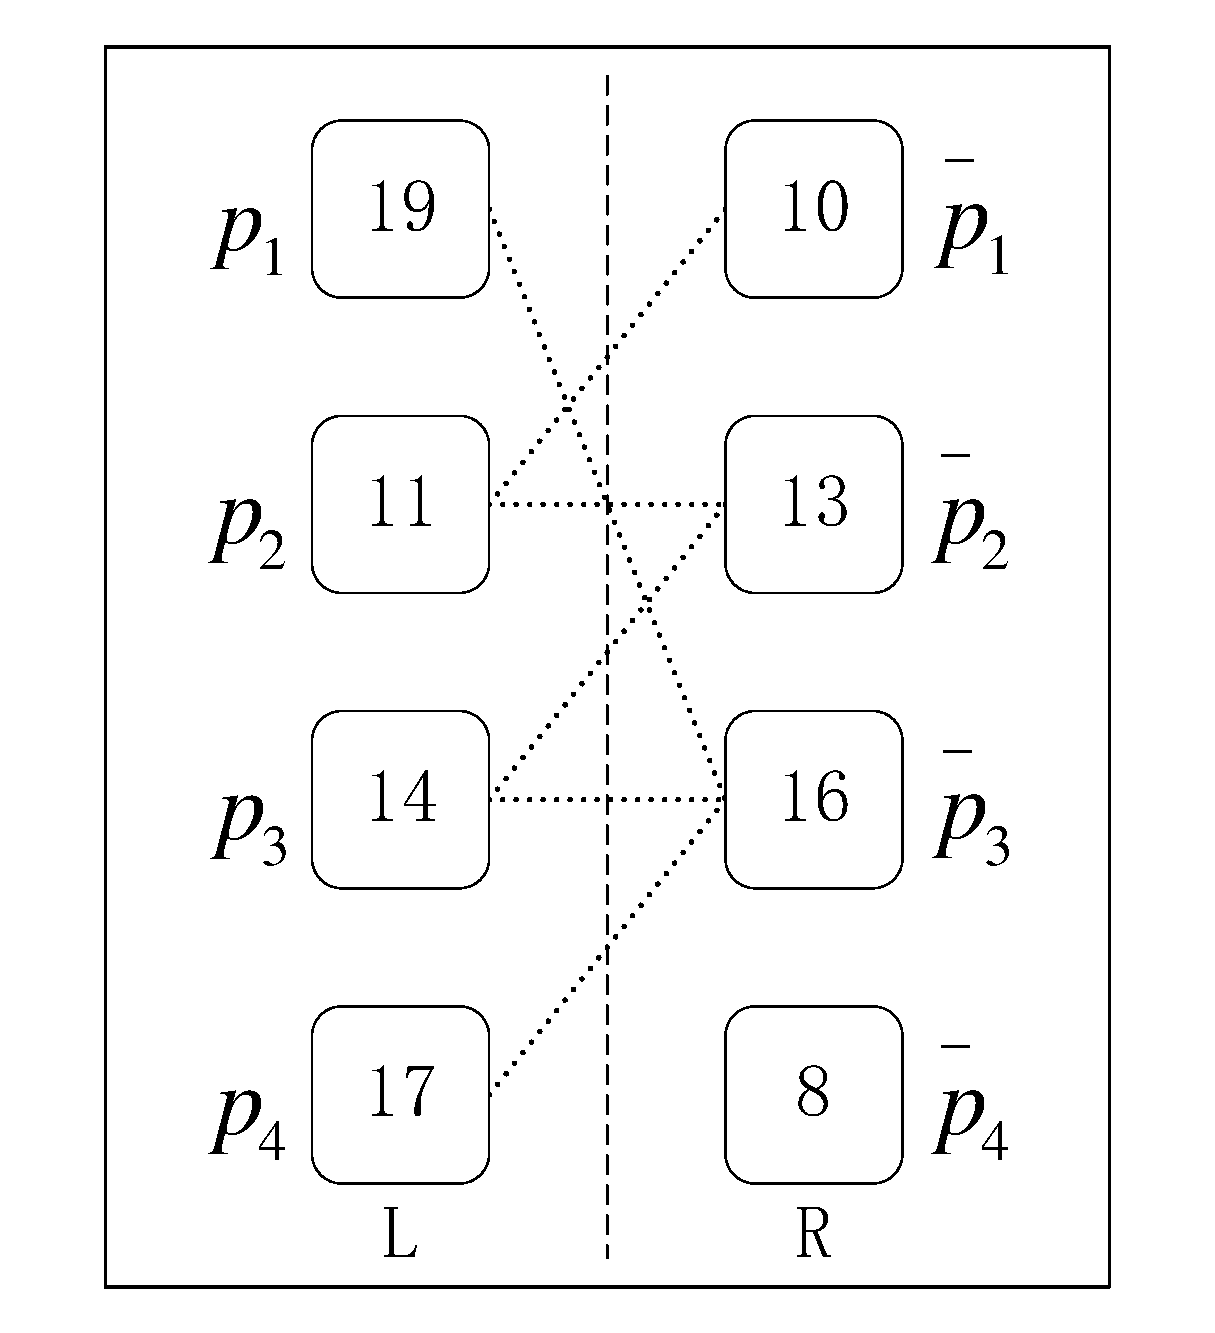
\includegraphics[width=0.32\columnwidth]{fig/bi1.eps}
   }
   \subfigure[二部图匹配结果。 匹配对用实线连接。]
   {
     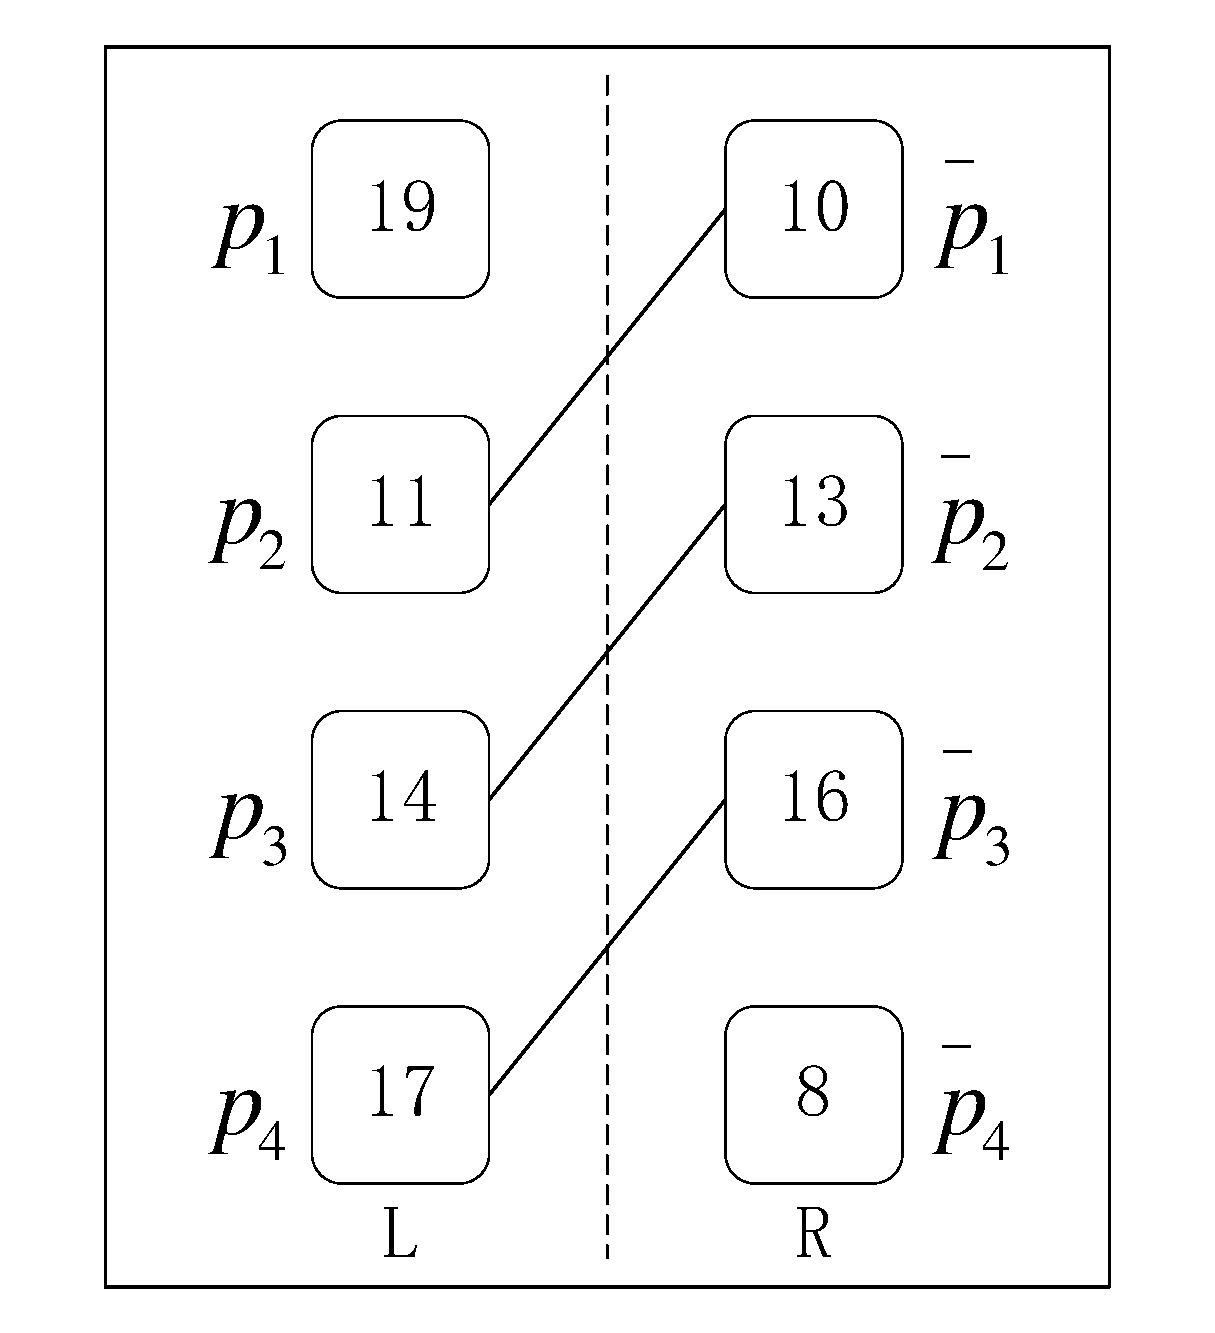
\includegraphics[width=0.32\columnwidth]{fig/bi2.eps}
   }
   \caption{带权重二部图匹配的例子}\label{fig:bi2}
 \end{figure}
 






























